\documentclass[11pt,fleqn]{article}

\textheight=23.3cm
\textwidth=16.5cm
\topmargin=-15mm
\oddsidemargin=0cm

\usepackage{enumerate}
\usepackage{amsmath}
\usepackage{amssymb}
\usepackage{bbm}
\usepackage{graphicx}
\usepackage{wrapfig}
\usepackage{pdflscape}
\usepackage[sidewaysfigure]{rotating}
\usepackage{natbib}
\usepackage{multirow}
\newcommand{\tb}{\hspace*{3mm}}
\bibpunct{(}{)}{;}{a}{,}{,}
\parskip=3mm
\parindent=5mm
\baselineskip=17pt

\usepackage{amsthm}
\newtheorem{assumption}{Assumption}
\newtheorem{definition}{Definition}
\newtheorem{proposition}{Proposition}

\DeclareMathOperator*{\argmax}{arg\,max}
\DeclareMathOperator*{\argmin}{arg\,min}

\usepackage{hyperref}
\hypersetup{
  pdftitle={Laun \& Wallenius (2015) - A Life Cycle Model of Health and Retirement: Swedish Pension Reform},
  pdfauthor={Robert Kirkby},
  colorlinks=true,
  linkcolor=black,
  citecolor=black,
  urlcolor=blue,
  breaklinks=true
}


\begin{document}

\title{Laun \& Wallenius (2015) - A Life Cycle Model of Health and Retirement: Swedish Pension Reform}
\author{Robert Kirkby}
\date{\today}
\maketitle

A full replication of \citet{LaunWallenius2015}, hereafter LW2015. This document describes how the model is expressed in terms of the VFI Toolkit. For the full description, motivation, and policy results see the original paper.

We solve all of LW2015's main model exercises: the pre-reform Swedish economy as baseline; the regular-only pension reform in both partial and general equilibrium; the full reform (regular pension + occupational pension reform) in both partial and general equilibrium; and the per-PType welfare consumption-equivalent variation. One unavoidable departures remain: the wage profiles are eyeballed humps from LW2015 Fig.\ 1.\footnote{A related paper \citet{LaunWallenius2016} for which code is available only has two profiles instead of LW2015's four, so we cannot borrow}

The wage profiles are based on regression coefficients that are not published anywhere we can locate, and recreating the regressions would require access to the Swedish LINDA database. We do not reperform the calibration exercise as the targets are not available, and recreating them would again require access to the Swedish LINDA database.


\section{Model description}
The model is a discrete-time, finite-horizon, life-cycle model with permanent skill heterogeneity. Agents are model period $j=0,\ldots,55$ (real-life age $25,\ldots,80$) and live with certainty to age $80$. Each period an agent of skill type $s$ chooses consumption $c$, asset holdings $k'$, indivisible labor $l\in\{0,\bar l\}$ (with $\bar l = 1/3$), and -- subject to eligibility -- whether to apply for disability insurance (DI) and/or claim the regular pension benefit (PB). The agent receives an exogenous shock to health, $h\in\{1,\ldots,5\}$ (very bad through very good).

Preferences are
\begin{equation*}
 \sum_{j=0}^{55} \beta^{\,j} \left[ \ln c_{j,s} - b(h_{j,s})\, l_{j,s} + h_{j,s} \right],
\end{equation*}
with $\beta=1/(1+r)$ and disutility from work $b(h)$ decreasing in health (LW2015 Table 4). The budget constraint is
\begin{equation*}
 (1+\tau_c)\, c + k' = (1+r)\, k + (1-\tau_y(Y))\, Y - \tau_{ss}\, w_{j,s} l + T,
\end{equation*}
with $Y = w_{j,s} l + \text{DI} + \text{PB} + \text{OPB}$ total taxable income, $\tau_y(\cdot)$ the two-bracket progressive labor income tax (rates $\tau_{\ell1}, \tau_{\ell2}$), $\tau_{ss}$ the social-security payroll tax, $\tau_c$ the consumption tax, and $T$ a lump-sum transfer. Wages $w_{j,s}$ are deterministic, varying by model period $j$ and skill type $s$.

Health evolves as a Markov chain with age- and health-dependent transition probabilities (LW2015 Table 4): each period a small negative shock ($h\to h-1$), a large negative shock ($h\to h-3$), or a positive shock ($h\to h+1$) may hit. When the three event probabilities sum to more than one we renormalize them to sum to one (no ``stay'' mass); otherwise the residual is ``stay''.

DI claiming requires health $\le 2$ (bad/very bad); once on DI the agent stops working and remains on DI until age 65, at which point DI converts to PB. PB can be claimed from age 61. Both claim events are absorbing. Occupational pension (OPB) is collected from age 65 if the agent is still working at 65, or earlier (from age 55) if the agent has already stopped working --- with a 0.6\%-per-month actuarial reduction for early-claiming white-collar workers, and a 0.7\%-per-month bonus for delayed claiming by blue-collar workers up to age 70.

\subsection*{Wage profiles --- a flagged departure from the paper}\label{sec:wage-profiles}
LW2015 estimates four age-earnings profiles $w_{j,s}$ from the LINDA panel (1968--1997) by regressing annual earnings on age, age$^2$, and individual fixed effects. The four profiles correspond to the four PTypes: non-college / college $\times$ low / high productivity, where low/high within each education group is the fixed-effect dimension. The paper plots them in Fig.~1 but does not print the regression coefficients in the article, in the SSE working-paper version (WP 741), in any online appendix, or in any replication package we can locate. The Journal of Public Economics article has no supplementary materials section; the authors' homepages have no replication code; the working-paper directory has no appendix.

We tried to borrow from the LW2016 sequel paper's replication code (RED Computer Codes 14-161 at \texttt{https://red-files-public.s3.amazonaws.com/codes/14/14-161/CodeZIP.zip}), which \emph{does} publish a regressed wage profile in \texttt{Compusswe/Version~1/w.m}. That file would let us avoid eyeballing if it had four profiles. It has only two: high school and college. The within-education fixed-effect dimension --- the part that distinguishes LW2015's NCL from NCH, and CL from CH --- was dropped in the LW2016 model, which redirects the heterogeneity into a separate disutility-of-work preference parameter. Using the LW2016 two profiles for our four PTypes (by either duplicating each across its low/high split, or fabricating a productivity premium) would either lose half the heterogeneity or require a number not in any source. We chose not to do either.

What we do instead: read the four profiles off LW2015 Fig.~1 as carefully as we can, fit hump-shaped quadratics
\[ w_s(j) = w_{\text{low},s} + (w_{\text{peak},s} - w_{\text{low},s}) \cdot \max\!\left\{0,\; 1 - ((j + \texttt{agejshifter} - 50)/30)^2\right\} \]
with $(w_{\text{low}}, w_{\text{peak}})$ in BA/year set to NCL $(2.0, 3.5)$, NCH $(3.0, 5.0)$, CL $(3.0, 5.5)$, CH $(5.0, 10.0)$. Each quadratic peaks at real age 50 (model period $j = 26$). The choice of $30$ in the denominator controls the curvature width --- chosen so the profiles return to roughly the low values at ages 25 and 75 in line with Fig.~1.

These four pairs are the single biggest source of irreducible uncertainty in the replication. Everything else in the model is calibrated directly from numbers printed in the paper. If LINDA access is available, the actual regression coefficients should be re-estimated by running the same age, age$^2$, fixed-effect regression on Swedish panel data 1968--1997 and substituting the resulting four quadratic profiles into \texttt{Params.w\_low\_i} and \texttt{Params.w\_peak\_premium\_i} in the driver. The replication is otherwise structurally complete.




\section{Replication Results}
Figures \ref{fig:LW2015_fig1} was based on data in the original paper, we here show the model version as these are the 'age profiles of earnings' that we had to eyeball from the graph, so we want to see they look okay.

Figures \ref{fig:LW2015_fig3} and \ref{fig:LW2015_fig4} show the resulting model employment rate and DI incidence by 5-year age bin -- the model line of LW2015 Figures 3 and 4. The data line is not reproduced here.


\begin{figure}[htp]
\centering
\includegraphics[width=140mm]{../SavedOutput/Graphs/LuanWallenius2015_Figure1.png}
\caption{LW2015 Fig 1: life cycle earnings of Swedish males by skill type. Hump-shaped quadratics with $(w_{\text{low}}, w_{\text{peak}})$ eyeballed from the paper's Fig 1; see the calibration shortcuts section for the disclaimer that the underlying LINDA regression coefficients are not published.}
\label{fig:LW2015_fig1}
\end{figure}

\begin{figure}[htp]
\begin{center}
\begin{tabular}{c}
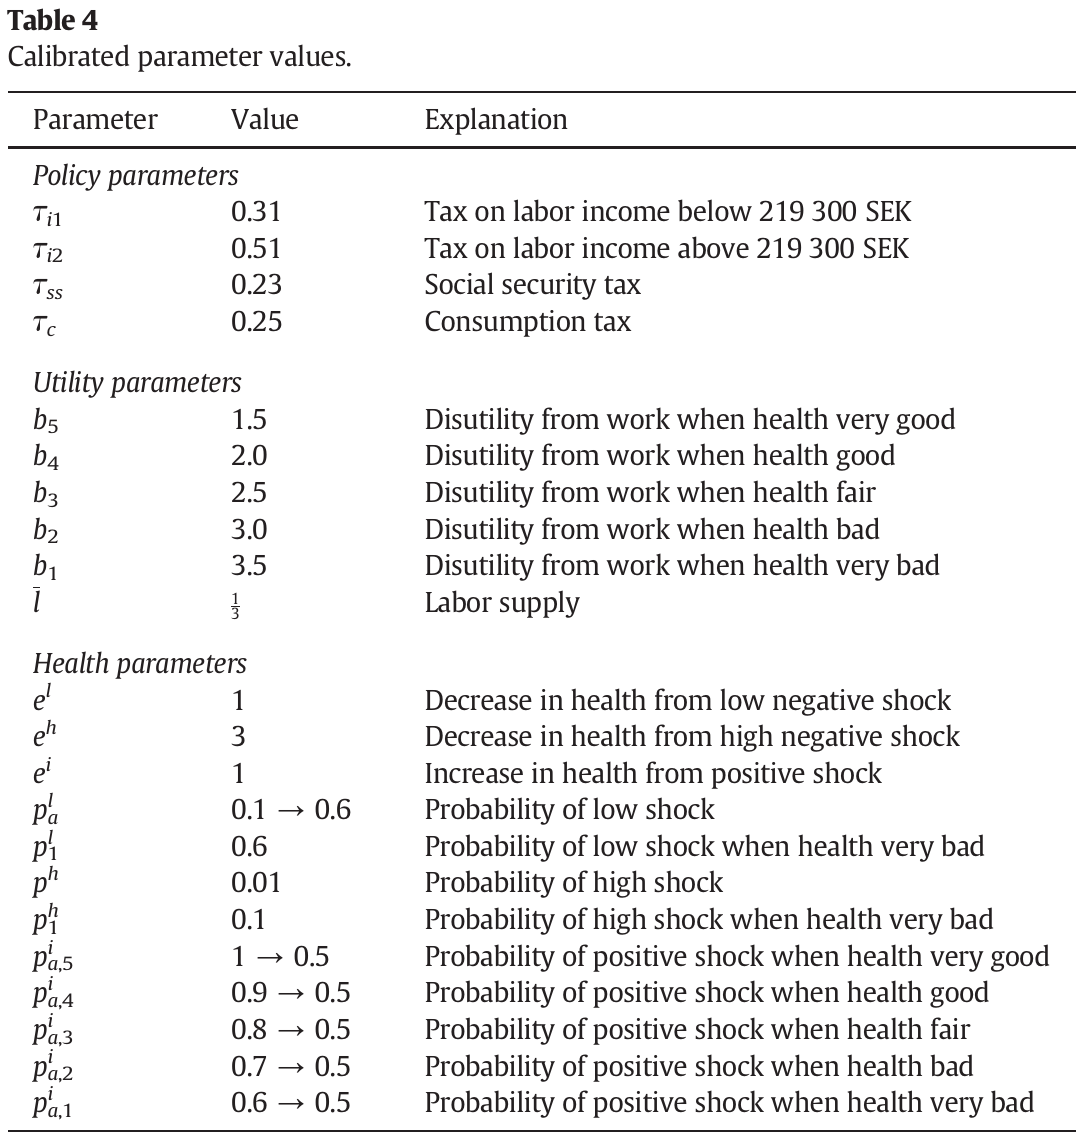
\includegraphics[width=120mm]{./OriginalMaterials/LW2015_OriginalTable4.png}
\end{tabular}
\end{center}
\begin{center}
\begin{tabular}{c}
\input{../SavedOutput/LatexInputs/LuanWallenius2015_Table4.tex}
\end{tabular}
\end{center}
\caption{Table 4 of LW2015 (top), replication generated from the driver's \texttt{Params} struct (bottom).}
\label{tab:LW2015_table4}
\end{figure}

\begin{figure}[htp]
\begin{center}
\begin{tabular}{c}
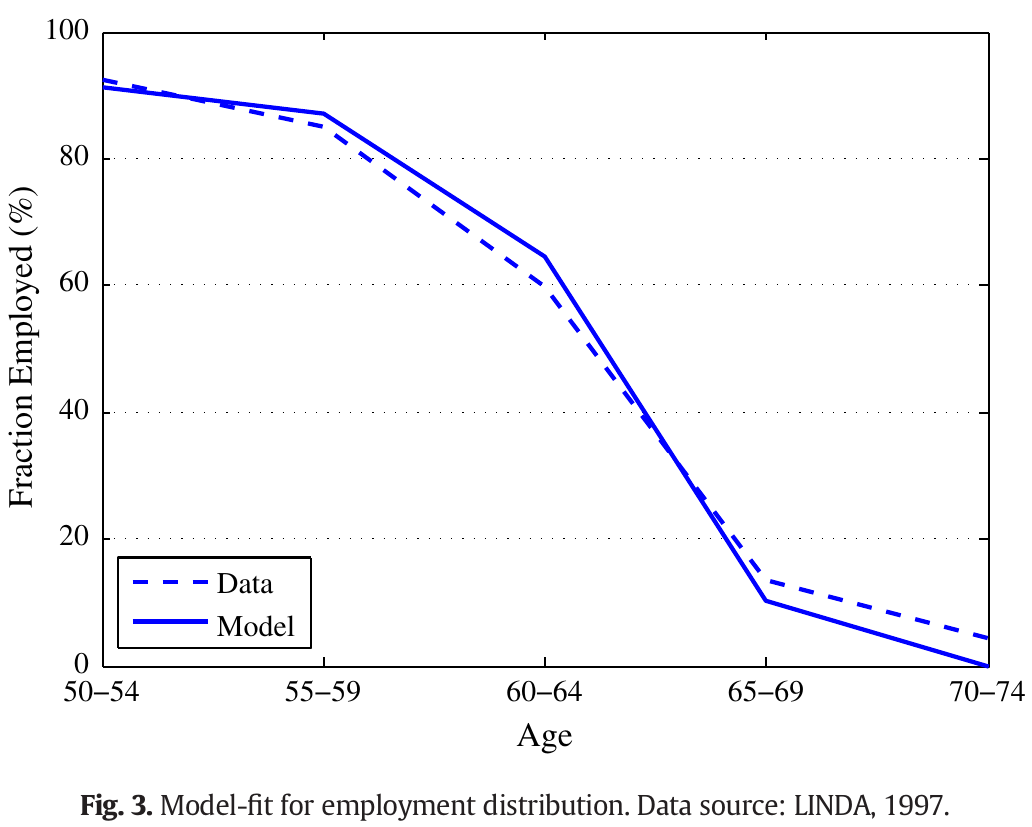
\includegraphics[width=120mm]{./OriginalMaterials/LW2015_OriginalFigure3.png} \\
\includegraphics[width=140mm]{../SavedOutput/Graphs/LuanWallenius2015_Figure3.png}
\end{tabular}
\end{center}
\caption{Figure 3 of LW2015 (top), replication (bottom): fraction employed by age bin, pre-reform calibration. Pop-weighted across PTypes; averaged within each 5-year bin. We only reproduce the model line.}
\label{fig:LW2015_fig3}
\end{figure}

\begin{figure}[htp]
\begin{center}
\begin{tabular}{c}
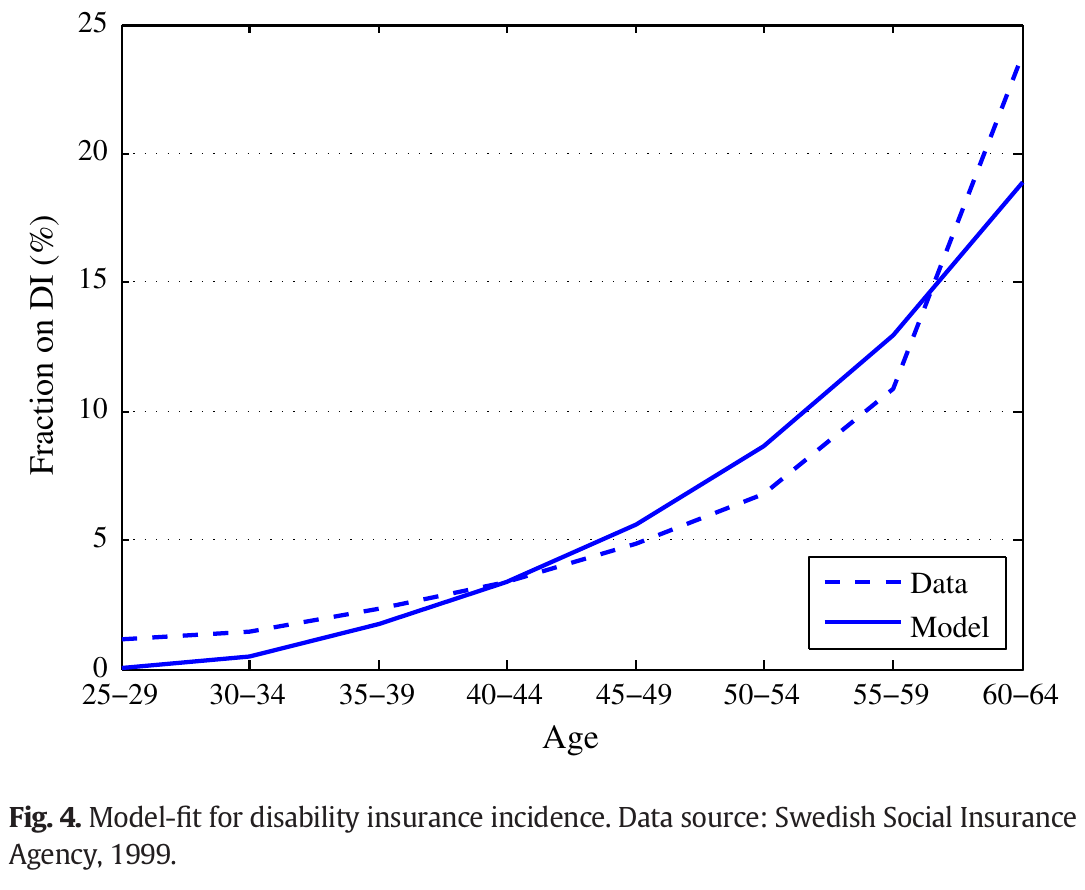
\includegraphics[width=120mm]{./OriginalMaterials/LW2015_OriginalFigure4.png} \\
\includegraphics[width=140mm]{../SavedOutput/Graphs/LuanWallenius2015_Figure4.png}
\end{tabular}
\end{center}
\caption{Figure 4 of LW2015 (top), replication (bottom): disability-insurance incidence by age bin, pre-reform calibration. Pop-weighted across PTypes; averaged within each 5-year bin. We only reproduce the model line.}
\label{fig:LW2015_fig4}
\end{figure}

\begin{figure}[htp]
\begin{center}
\begin{tabular}{c}
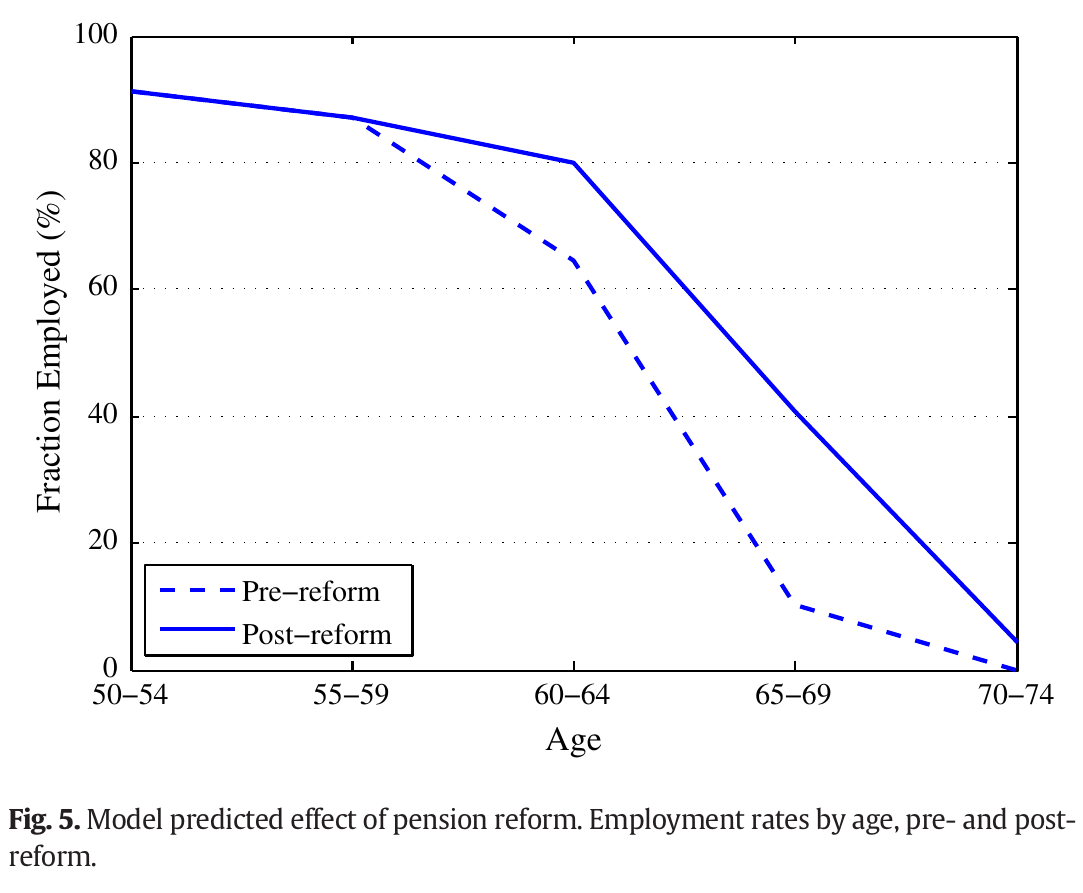
\includegraphics[width=120mm]{./OriginalMaterials/LW2015_OriginalFigure5.png} \\
\includegraphics[width=140mm]{../SavedOutput/Graphs/LuanWallenius2015_Figure5.png}
\end{tabular}
\end{center}
\caption{Figure 5 of LW2015 (top), replication (bottom): pre-reform vs full post-reform employment by age bin. Both lines under general equilibrium ($T$ solved as a price). This is the headline labor-supply result driving the +2.5-year retirement-age increase.}
\label{fig:LW2015_fig5}
\end{figure}

\begin{figure}[htp]
\centering
\includegraphics[width=140mm]{../SavedOutput/Graphs/LuanWallenius2015_Figure5b.png}
\caption{Our addition (not in LW2015): partial-equilibrium vs general-equilibrium employment under the regular-only pension reform. The two post-reform lines differ because of the GE $T$-adjustment.}
\label{fig:LW2015_fig5b}
\end{figure}

\begin{figure}[htp]
\begin{center}
\begin{tabular}{c}
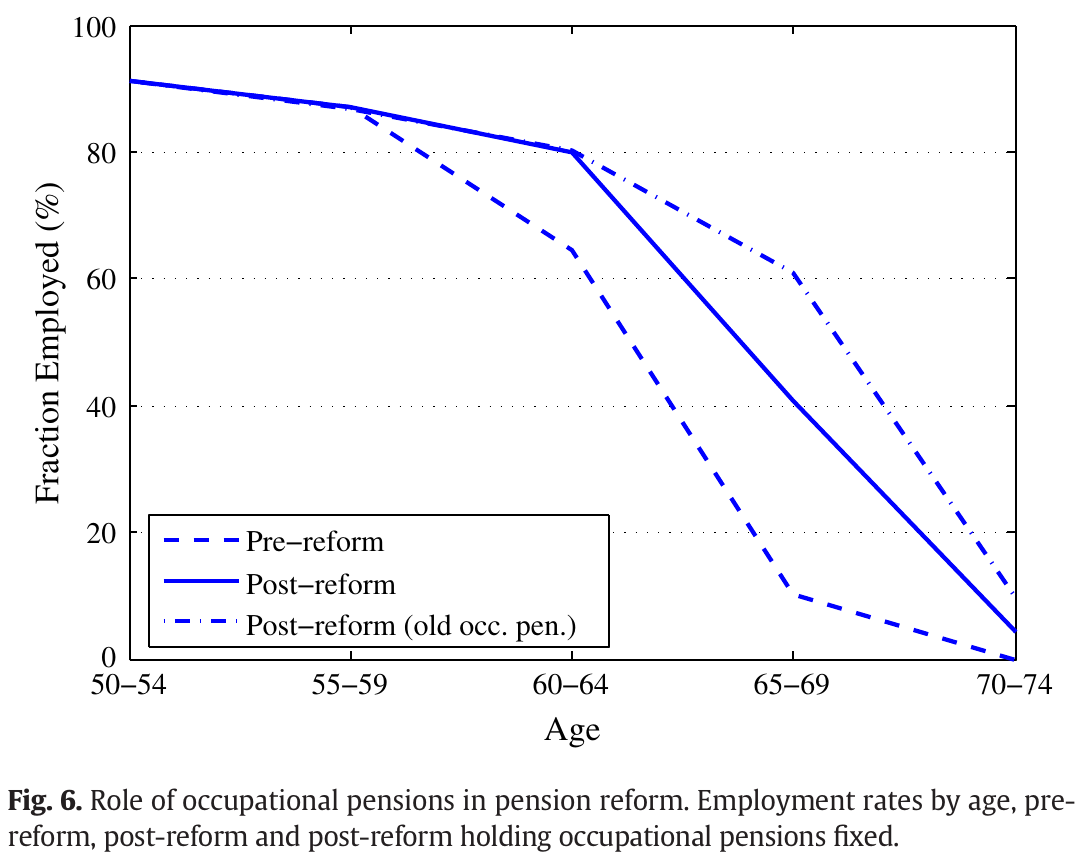
\includegraphics[width=120mm]{./OriginalMaterials/LW2015_OriginalFigure6.png} \\
\includegraphics[width=140mm]{../SavedOutput/Graphs/LuanWallenius2015_Figure6.png}
\end{tabular}
\end{center}
\caption{Figure 6 of LW2015 (top), replication (bottom): the role of the occupational-pension reform. Three lines: pre-reform; full reform (regular pension + occupational); and regular pension reform only (occupational pension held at pre-reform formula). Both post-reform lines under GE. The full-reform line sits below the regular-only line at 65--69 and 70--74 because the new DC occupational scheme is more generous, partly offsetting the work incentive from the NDC regular pension.}
\label{fig:LW2015_fig6}
\end{figure}

\newpage

\bibliographystyle{plainnat}
\bibliography{LuanWallenius}

\appendix

\section{Details on Model Implementation}\label{app:model-impl}

\subsection{State space in VFI Toolkit terms}
In VFI Toolkit notation the problem has

\begin{itemize}
\item \textbf{Permanent types} $N_i = 4$, \verb|Names_i = {NCL,NCH,CL,CH}|: non-college / college $\times$ low / high productivity (LW2015 Fig.~1). The first two PTypes are assigned to the blue-collar occupational pension scheme, the second two to white-collar.
\item \textbf{Decision variable} \verb|n_d = 5|: an action code dispatching joint labor / claim decisions; see Section~\ref{sec:histidx} for the enumeration.
\item \textbf{Standard endogenous states} \verb|n_a = [n_k, n_hist] = [300, 1237]|: assets $k\in[0,50\text{BA}]$ on 300 grid points, plus a single history-index $\text{hist\_idx}$ that encodes the agent's stop-work age, DI-claim age, and PB-claim age. $\text{hist\_idx}$ is the last entry of \verb|n_a| and is treated as the experienceasset (\verb|vfoptions.experienceasset=1|). Section~\ref{sec:histidx} explains in detail.
\item \textbf{Exogenous state} \verb|n_z = 5|: health $h\in\{1,\ldots,5\}$, with age-dependent transition matrix \verb|pi_z_J| of shape $5\times 5\times N_j$.
\item $N_j = 56$, $\verb|agejshifter| = 24$.
\end{itemize}


\subsection{The \texttt{hist\_idx} experienceasset}\label{sec:histidx}

The single integer-valued state $\text{hist\_idx}\in\{1,\ldots,1237\}$ does the heavy lifting in this replication. It replaces what a more naive design would carry as four separate states: a DI-claim flag, a PB-claim flag, a stop-work-age tracker, and an Average Pension Points (AP) state. This section explains what $\text{hist\_idx}$ encodes, why each piece is needed to support the model's exercises, why we use a compact encoding rather than the unconstrained cartesian product, and how the integer is unpacked and updated.

\subsubsection{What it encodes}

$\text{hist\_idx}$ packs three ``employment-history coordinates'' into a single integer:
\begin{align*}
 \text{swa} &\;=\;\text{first stop-work age}\quad\text{(model period; 0 = never stopped),}\\
 \text{dia} &\;=\;\text{first DI-claim age}\quad\text{(model period; 0 = never claimed DI),}\\
 \text{pba} &\;=\;\text{first PB-claim age}\quad\text{(model period; 0 = never claimed PB).}
\end{align*}
All three are absorbing. Work is absorbing once stopped (consistent with LW2015's ``each possible employment history'' phrasing, p.129, and explicit in the LW2016 replication code's loop structure). DI is absorbing pre-65 and converts mechanically to PB at age 65 with the same benefit amount, so no separate ``DI-then-PB'' flag is needed. PB is absorbing once claimed.

\subsubsection{Why each coordinate is needed}

A reasonable question is whether all three coordinates are necessary. They are not all logically independent (the reachable region in Section~\ref{sec:reach} shows the dependencies), but conceptually each one is the minimal carrier of information for one of the model's benefit formulas:

\begin{description}
 \item[swa is needed for both OPB and the post-reform NDC pension.] The pre-reform blue-collar OPB depends on average pension points from real ages 55--59 (LW2015 p.130) --- the relevant slice of the wage history is pinned by swa. The pre-reform white-collar OPB depends on ``income at the time of retirement'' (p.130), i.e.\ wage at swa$-1$. Most importantly, the post-reform NDC pension recalculates the benefit when the agent stops working (LW2015 p.133: \emph{``The benefit is then recalculated when the individual stops working''}), so swa is the AP-finalization age in the post-reform system. Without swa as state, this rule cannot be implemented.
 \item[dia is needed for DI and the OPB DI top-up.] The DI benefit in both pre- and post-reform systems uses an AP projection that extends the ``contributing-years denominator'' to age 65 by filling in projected years at the rate of the last 3 pre-DI years (LW2015 p.131). That projection depends on \emph{when} DI was claimed, not just on the current age. The OPB DI top-up (LW2015 p.131; 15\% of pre-DI wage plus white-collar brackets) similarly depends on wage at dia$-1$, i.e.\ on dia.
 \item[pba is needed for the PB actuarial adjustment.] LW2015 p.130: $-0.5$\%-points per month early for the regular pension, $+0.7$\%/month delayed. That schedule is a function of the \emph{claim} age, which can differ from the stop-work age (the model allows claiming PB while still working).
\end{description}

These three are exactly the indices LW2016's hand-rolled code carries (\verb|i0, i1, i2| in lch1.m of the RED archive), and they are what the LW2015 paper's prose on p.129 (``\emph{for each possible employment history, consisting of disability, pension and retirement decisions}'') refers to.

\subsubsection{Reachable region}\label{sec:reach}

The unconstrained cartesian product of $(\text{swa}, \text{dia}, \text{pba})$ has $57 \times 41 \times 21 = 49{,}077$ entries:
\begin{itemize}
 \item swa ranges over $\{0,1,\ldots,56\}$ --- 56 model ages plus the sentinel 0 for ``never stopped''.
 \item dia ranges over $\{0, 1, \ldots, 40\}$ --- model ages 1--40 (real ages 25--64, the legal DI-claim window) plus 0 for ``never''.
 \item pba ranges over $\{0, 37, 38, \ldots, 56\}$ --- model ages 37--56 (real ages 61--80, the legal PB-claim window) plus 0 for ``never''.
\end{itemize}
But the model's structural constraints rule out the vast majority of this product. Two facts do the work:

\begin{enumerate}
 \item Work is absorbing once stopped, and DI implies stop-work (the agent cannot work on DI). So whenever dia $\ne 0$, we have $\text{swa} = \text{dia}$ --- one degree of freedom collapses.
 \item DI and PB are mutually exclusive pre-65, and the 65-conversion is mechanical (no separate PB-claim event). So on the DI branch, $\text{pba} = 0$ always.
\end{enumerate}

The reachable region therefore splits into two contiguous blocks:

\begin{itemize}
 \item \textbf{Block A (no DI ever):} $\text{dia} = 0$, with $(\text{swa}, \text{pba})$ varying freely over $\{0,\ldots,56\} \times \{0, 37, \ldots, 56\}$. That is $57 \times 21 = 1197$ tuples.
 \item \textbf{Block B (DI claimed):} $\text{dia} \in \{1,\ldots,40\}$, with $\text{swa} = \text{dia}$ (forced) and $\text{pba} = 0$. That is $40$ tuples.
\end{itemize}

Total reachable: $1197 + 40 = 1237$ tuples, about 2.5\% of the unconstrained product.

\subsubsection{The integer encoding}

We map the reachable region to integers $\{1,\ldots,1237\}$ by laying the two blocks out contiguously:

\paragraph{Block A (indices 1--1197).} Define $\text{pba\_idx} = 1$ if $\text{pba} = 0$, else $\text{pba\_idx} = \text{pba} - 35$ (giving $\text{pba\_idx}\in\{1,\ldots,21\}$). Then
\[
 \text{hist\_idx} \;=\; \text{swa} \cdot 21 + \text{pba\_idx}.
\]

\paragraph{Block B (indices 1198--1237).}
\[
 \text{hist\_idx} \;=\; 1197 + \text{dia}.
\]

\paragraph{Decoding.} Given $\text{hist\_idx}$:
\begin{itemize}
 \item If $\text{hist\_idx} \le 1197$:
 \begin{align*}
  \text{swa} &= \lfloor (\text{hist\_idx}-1)/21 \rfloor, \\
  \text{pba\_idx} &= ((\text{hist\_idx}-1) \bmod 21) + 1, \\
  \text{pba} &= \begin{cases} 0 & \text{if } \text{pba\_idx} = 1 \\ \text{pba\_idx} + 35 & \text{otherwise}\end{cases},\\
  \text{dia} &= 0.
 \end{align*}
 \item Otherwise (DI branch):
 \begin{align*}
  \text{dia} &= \text{hist\_idx} - 1197,\quad \text{swa} = \text{dia},\quad \text{pba} = 0.
 \end{align*}
\end{itemize}

The encode/decode arithmetic is duplicated inline in \verb|LuanWallenius2015_aprimeFn.m| and \verb|LuanWallenius2015_ReturnFn.m|. Factoring it into a helper file would be slightly cleaner but would prevent toolkit-side inlining --- both of those functions are on the inner loop of the value-function iteration and called millions of times.

\subsubsection{The decision variable d and the transition rule}

The decision $d \in \{1, 2, 3, 4, 5\}$ enumerates joint labor / claim actions:
\begin{itemize}
 \item $d=1$: keep working, no claim change. Feasible only if $\text{swa} = 0$ and the agent is not on DI.
 \item $d=2$: stop working (or stay stopped), no claim change. Always feasible; forced choice when on DI.
 \item $d=3$: apply for DI (forces stop work). Feasible only if $\text{dia} = 0$, $\text{agej} \le \text{agej\_di\_max}$, $\text{pba} = 0$, and $h \le 2$.
 \item $d=4$: claim PB and stop working. Feasible only if $\text{pba} = 0$, $\text{agej} \ge \text{agej\_pb\_first}$, and $\text{dia} = 0$.
 \item $d=5$: claim PB and keep working. Same as $d=4$ but also requires $\text{swa} = 0$.
\end{itemize}
Eligibility constraints are enforced inside the return function (\verb|LuanWallenius2015_ReturnFn.m|) by returning $-\infty$ for infeasible $(d, \text{state})$ pairs; the aprimeFn just executes the formal transition without checking eligibility, knowing that infeasible-action paths will be excluded by $-\infty$ utilities.

\paragraph{aprimeFn.} The history-state transition is a pure function of $(d, \text{hist\_idx}, \text{agej})$:
\begin{enumerate}
 \item Decode $\text{hist\_idx} \to (\text{swa}, \text{dia}, \text{pba})$.
 \item Apply the $d$-specific update rule:
\begin{align*}
 d=1: &\quad (\text{swa}', \text{dia}', \text{pba}') = (\text{swa}, \text{dia}, \text{pba}). \\
 d=2: &\quad \text{swa}' = \begin{cases}\text{agej} & \text{if swa}=0 \\ \text{swa} & \text{otherwise}\end{cases},\; \text{dia}'=\text{dia},\; \text{pba}'=\text{pba}.\\
 d=3: &\quad \text{if feasible: } (\text{swa}', \text{dia}', \text{pba}') = (\text{agej}, \text{agej}, \text{pba}). \\
 d=4: &\quad \text{if feasible: } \text{pba}' = \text{agej},\; \text{swa}' = \max(\text{swa}, \text{agej})|_{\text{first-stop}},\; \text{dia}'=\text{dia}. \\
 d=5: &\quad \text{if feasible: } \text{pba}' = \text{agej},\; \text{swa}' = \text{swa},\; \text{dia}'=\text{dia}.
\end{align*}
 (Where ``if feasible'' means the eligibility test in the action description above; otherwise the state is left unchanged --- the $-\infty$ utility in the return function makes this branch ignored by the argmax.)
 \item Encode $(\text{swa}', \text{dia}', \text{pba}') \to \text{hist\_idx}'$.
\end{enumerate}

\paragraph{Toolkit plumbing.} Because the transition depends only on the experienceasset, the decision, and the age --- not on $z$ or any other state --- this fits the plain experienceasset signature:
\begin{verbatim}
vfoptions.experienceasset = 1;
vfoptions.aprimeFn = @(d, hist_idx, agej, agej_pb_first, agej_di_max) ...
                     LuanWallenius2015_aprimeFn(d, hist_idx, agej, ...
                                                agej_pb_first, agej_di_max);
\end{verbatim}
Because the grid \verb|hist_grid = (1:1237)'| is integer-valued and the aprimeFn always returns an exact grid point, the toolkit's experienceasset lottery degenerates to a point mass at every transition --- no interpolation occurs, no precision is lost, and the policy function lives on the natural integer grid.

\subsubsection{Benefits as on-the-fly functions of \texttt{hist\_idx}}

All five benefit calculations (AP, PB, DI, OPB, OPB-DI-top-up) are pure functions of the decoded $(\text{swa}, \text{dia}, \text{pba})$ plus current age and PType-specific wage parameters. They are \emph{not} precomputed into matrices; instead, each lives in its own \verb|.m| file (\verb|LuanWallenius2015_AP.m|, \verb|_PB.m|, \verb|_DI.m|, \verb|_OPB.m|, \verb|_OPB_DI.m|) and is invoked by the return function. The AP function in particular implements the literal top-15-best rule from LW2015 p.130, with the 3-year-pre-DI projection that LW2015 p.131 describes for DI claimants (matching LW2016's \verb|penpoints.m|). The OPB and OPB-DI formulas implement the blue/white-collar piecewise rules from LW2015 p.130--131, including the 0.6\%/month early-claim reduction for white-collar and the 0.7\%/month late-claim bonus for blue-collar (LW2016 \verb|Toccl.m|, \verb|Tochs.m|, \verb|Tdioc.m|).

The runtime cost is an $O(N_j)$ pass through the wage profile inside each return-function call. A later optimization pass could lift each benefit into a precomputed lookup table indexed by $(\text{swa}, \text{dia}, \text{pba}, \text{PType}, \text{agej})$ without changing the public function signatures --- but for the current replication clarity wins over speed.

\subsubsection{Initial distribution}

All agents begin at $\text{hist\_idx} = 1$, which decodes to $\text{swa} = 0$, $\text{dia} = 0$, $\text{pba} = 0$ (``never claimed anything''). Combined with $k = 0$ and $h = 5$ (very good), this matches the paper's initial condition --- LW2015 p.129: \emph{``All agents start out with zero capital and in very good health.''}


\subsection{Health-transition Markov chain}\label{sec:health}

LW2015 Table~4 specifies three exogenous health shocks but does not aggregate them into an explicit one-step Markov transition. We work out the interpretation here.

\subsubsection{The three shocks}

Each period each agent draws:
\begin{itemize}
 \item a small negative shock, $\Delta h = -1$, with probability $p^l$;
 \item a large negative shock, $\Delta h = -3$, with probability $p^h$;
 \item a positive shock, $\Delta h = +1$, with probability $p^i$.
\end{itemize}
$p^l$ rises linearly in age from $0.1$ at age 25 to $0.6$ at age 80, with the LW2015 Table 4 override $p^l_1 = 0.6$ (constant) at $h=1$. $p^h$ is constant $0.01$, with override $p^h_1 = 0.1$ at $h=1$. $p^i$ varies with both age and health: it falls linearly from $\{0.6, 0.7, 0.8, 0.9, 1.0\}$ for $h \in \{1, 2, 3, 4, 5\}$ at age 25 to $0.5$ at age 80.

\subsubsection{The aggregation ambiguity}

The paper does not say how the three shock probabilities combine into a Markov transition $\pi_z(h \to h')$. The natural reading is ``one of the three events fires, residual $1 - p^l - p^h - p^i$ is no change''. But at several $(h, \text{age})$ cells the three probabilities sum to more than 1:
\begin{center}
\begin{tabular}{lccc}
 & $p^l$ & $p^h$ & $p^i$ \\
\hline
young $h=4$ & $0.10$ & $0.01$ & $0.90$ \\
old $h=4$   & $0.60$ & $0.01$ & $0.50$ \\
old $h=3$   & $0.60$ & $0.01$ & $0.50$
\end{tabular}
\end{center}
At each of these the three numbers cannot simultaneously be transition probabilities of mutually exclusive events. The mutually-exclusive reading therefore requires ad-hoc clipping or renormalization, both of which throw away ``stay'' mass at exactly the ages and health states most relevant for the paper's results.

\subsubsection{Reading A --- independent Bernoulli draws}

We adopt instead the reading that the three shocks fire \emph{independently}. Each period each shock fires (Bernoulli) with its Table-4 probability; the realized $\Delta h$ is the algebraic sum of the firing shock values; the new health state is the cap $h' = \max(1, \min(5, h + \Delta h))$.

The joint distribution has $2^3 = 8$ outcomes. For a given $(h, p^l, p^h, p^i)$:
\begin{center}
\begin{tabular}{lccc}
event combination & probability & $\Delta h$ & $h'$ \\
\hline
none                 & $(1-p^l)(1-p^h)(1-p^i)$           & $0$  & $h$ \\
only $p^l$           & $p^l(1-p^h)(1-p^i)$               & $-1$ & $\max(h-1, 1)$ \\
only $p^h$           & $(1-p^l)p^h(1-p^i)$               & $-3$ & $\max(h-3, 1)$ \\
only $p^i$           & $(1-p^l)(1-p^h)p^i$               & $+1$ & $\min(h+1, 5)$ \\
$p^l$ and $p^h$      & $p^l p^h (1-p^i)$                 & $-4$ & $1$ \\
$p^l$ and $p^i$      & $p^l (1-p^h) p^i$                 & $0$  & $h$ \\
$p^h$ and $p^i$      & $(1-p^l) p^h p^i$                 & $-2$ & $\max(h-2, 1)$ \\
all three            & $p^l p^h p^i$                     & $-3$ & $\max(h-3, 1)$
\end{tabular}
\end{center}
The transition $\pi_z(h \to h')$ is the sum of all event probabilities whose net change lands at $h'$. The resulting matrix is denser than under the mutually-exclusive reading --- every $h \to h'$ within four-step reach has positive mass, not just the three the table's headline numbers suggest --- but it requires no clipping and uses every published probability at face value.

\subsubsection{Qualitative consequences}

The independent-draw structure gives the positive shock a partial ``shield'' role. At $h=5$ young, $p^i = 1.0$ means the positive shock fires every period with certainty. A coincident small negative shock then nets to $0$ (stay at $h=5$); a coincident large negative shock nets to $-2$ (lands at $h=3$ instead of $h=2$). At unhealthy states the same mechanism in reverse: at $h=1$ the elevated $p^l = 0.6$ doesn't move the agent through the cap, but it does eat into the positive-shock recovery rate because the joint event ``positive and small negative'' nets to $0$ (stay at $h=1$). Both effects produce health persistence at the boundary states, which the paper notes as a target on p.128.

\subsubsection{Why Reading A}

Reading A uses every Table-4 parameter at face value, requires no renormalization, has a clean derivation, and is the closest match to LW2016's stylistic preference for independent-event products: in [Compusswe/Version 1/lch1.m] the negative shocks $(p^l, p^h)$ and the (endogenous) investment-success probability $p_e$ are combined as $(1-p^l-p^h) \cdot p_e + \ldots$ --- a literal joint-probability expansion of independent draws.

\subsubsection{Empirical validation}

The reading-choice question is settled directly against the paper's own reported model output: since health is purely exogenous in LW2015, the unconditional health distribution at any age is just the initial $P(h=5)=1$ propagated through $\pi_z$, independent of all other model parameters. LW2015 p.132 reports their model's distribution at real age 70 explicitly, and propagating under each reading gives an L1 distance to those numbers of $\mathbf{5.6}$ percentage points under Reading A vs $\mathbf{34.4}$ under Reading B. Reading A is decisively confirmed and Reading B ruled out. Appendix~\ref{app:health-test} reproduces the full propagation calculation, the test code, and the result table.


\subsection{Calibration shortcuts}

What we still depart from in the paper:

\begin{itemize}
\item \textbf{Wage profiles.} The four life-cycle earnings profiles in LW2015 Fig.~1 (LINDA 1968--1997) are estimated by regression on age, age$^2$, and individual fixed effects, but the regression coefficients are not printed in the paper, the SSE working-paper version (WP 741), or any online appendix or replication package we can locate. We \emph{cannot} borrow from the LW2016 sequel replication code (RED 14-161) either, because LW2016 publishes only \emph{two} regressed wage profiles in \verb|Compusswe/Version 1/w.m| (high school and college) --- the within-education fixed-effect dimension that LW2015 uses for the NCL/NCH and CL/CH split was dropped in LW2016. Pending either the original LW2015 LINDA regression output or LINDA access to re-estimate, we eyeball four hump-shaped quadratics from Fig.~1 with peak at real age 50; see the discussion in Section~\ref{sec:wage-profiles} for details.
\item \textbf{Lump-sum transfer in the pre-reform baseline.} Held at $T = 0.4\,\text{BA}$ (the paper's reported equilibrium value; $\approx 15{,}000$ SEK / 36{,}300 SEK $\approx 0.4\,\text{BA}$) rather than re-derived via a budget-balance loop. For the post-reform regimes $T$ is solved as a GE price via the toolkit's \texttt{HeteroAgentStationaryEqm\_Case1\_FHorz\_PType} with an inline \texttt{GeneralEqmEqns.budget = @(surplus, T) surplus - T}; see \texttt{doPart(3)} (regular-only GE) and \texttt{doPart(5)} (full reform GE) in the driver.
\item \textbf{Disutility-from-work and health-shock probabilities.} Set to LW2015 Table 4 values; not yet jointly recalibrated to match the employment and DI-incidence age profiles (LW2015 Tables 1--2).
\item \textbf{PType mass.} Set to LW2015's 17\% college / 83\% non-college sample share, split 50/50 low/high within each education group: $(0.415, 0.415, 0.085, 0.085)$.
\end{itemize}

What is now done at full paper fidelity (where the earlier draft of this replication had simplified):
\begin{itemize}
\item AP is the literal top-15-best rule with 3-year-pre-DI projection.
\item PB benefit includes the $\min(\text{yrs}/30,1)$ proration and the $\pm 0.5/0.7\%$/month actuarial adjustment.
\item DI benefit includes the projection-to-65 ``assumed pension points'' rule.
\item OPB supports early claim from age 55 for white-collar with the 0.6\%/month reduction, and late-claim bonus for blue-collar to age 70.
\item OPB DI top-up paid alongside DI (15\% of pre-DI wage for blue-collar; white-collar piecewise).
\end{itemize}

The next step in this replication would be (i) regressing the wage profiles from a comparable Swedish micro-dataset, and (ii) jointly calibrating the disutility levels $b(h)$ and the health-shock probabilities to match the employment and DI-incidence age profiles in LW2015 Tables 1--2 (the targets the paper itself calibrates to).


\section{Resolving the health-transition aggregation ambiguity}\label{app:health-test}

This appendix documents the test that pins down which aggregation reading the LW2015 authors used for the three exogenous health shocks. It is self-contained: it duplicates the basic setup of Section~\ref{sec:health} so a reader of just the appendix has the full picture.

\subsection*{The ambiguity}

LW2015 specifies that each period an agent receives up to three exogenous health shocks: a small negative shock ($\Delta h = -1$) with probability $p^l$, a large negative shock ($\Delta h = -3$) with probability $p^h$, and a positive shock ($\Delta h = +1$) with probability $p^i$. The values in LW2015 Table~4:
\begin{itemize}
 \item $p^l$ rises linearly in age from $0.10$ at age 25 to $0.60$ at age 80, with the override $p^l_1 = 0.60$ (constant) at $h=1$.
 \item $p^h = 0.01$ (constant), with override $p^h_1 = 0.10$ at $h=1$.
 \item $p^i$ falls linearly in age, from $\{0.6, 0.7, 0.8, 0.9, 1.0\}$ for $h \in \{1, 2, 3, 4, 5\}$ at age 25 to $0.50$ at age 80.
\end{itemize}

The paper does not say how these three probabilities combine into a one-step Markov transition $\pi_z(h \to h')$. At several $(h, \text{age})$ cells the three sum to more than $1$ (young $h=4$: $0.10 + 0.01 + 0.90 = 1.01$; old $h=4$: $0.60 + 0.01 + 0.50 = 1.11$; old $h=3$: $0.60 + 0.01 + 0.50 = 1.11$), so they cannot all be probabilities of mutually exclusive events. Some aggregation rule is needed, and two natural ones disagree.

\subsection*{The two readings}

\textbf{Reading A --- independent Bernoulli draws.} The three shocks fire \emph{independently} each period. The joint distribution has $2^3 = 8$ outcomes; the realized $\Delta h$ is the algebraic sum of the firing shock values; the new health state is the cap $h' = \max(1, \min(5, h + \Delta h))$. This requires no clipping and uses every published parameter at face value, but produces a denser transition matrix where many $h \to h'$ pairs have positive mass (e.g.\ at $h=5$, mass can land at $h' \in \{5, 4, 3, 2, 1\}$ depending on which combinations fire).

\textbf{Reading B --- mutually exclusive with renormalization.} At most one of the three events fires per period; the residual $1 - p^l - p^h - p^i$ is ``stay''. When the three probabilities sum to more than $1$, they are rescaled to sum to $1$ (no ``stay'' mass remaining) and $p^i$ is forced to $0$ at $h=5$ (where the positive shock is a no-op at the upper cap anyway). This gives a sparser matrix --- at most three off-diagonal entries per row, plus a ``stay'' entry --- but discards stay-mass at exactly the ages where the paper's numbers overshoot.

\subsection*{The test}

LW2015 p.132 reports the model's own health distribution at real age 70:
\begin{quote}
\emph{``the model predicts that at age 70: 42\% of people are in very good health, 25\% in good health, 13\% in fair health, 9\% in bad health and 11\% in very bad health.''}
\end{quote}
Health is purely exogenous in LW2015 --- no mortality, no behavioral feedback into the Markov chain. So the unconditional health distribution at any age is just the initial distribution $P(h=5)=1$ at $j=1$ propagated through $\pi_z$ for 45 periods, independent of disutility, wages, taxes, benefits, and DI uptake. The (42, 25, 13, 9, 11) target therefore depends only on $\pi_z$.

We build $\pi_z$ under each reading, propagate, and compare. The full standalone test:

\begin{small}
\begin{verbatim}
% Standalone test discriminating Reading A vs Reading B for the
% LW2015 health-transition Markov chain.

clear

agejshifter=24;
N_j=80-agejshifter;
p_pos_young=[0.6 0.7 0.8 0.9 1.0];

%% Build pi_z_J under Reading A (independent Bernoulli draws)
pi_z_J_A=zeros(5,5,N_j);
for jj=1:N_j
    age_frac=(jj-1)/(N_j-1);
    for hh=1:5
        if hh==1
            p_l=0.6; p_h=0.1;
        else
            p_l=0.1+0.5*age_frac;
            p_h=0.01;
        end
        p_i=p_pos_young(hh)-(p_pos_young(hh)-0.5)*age_frac;

        for s_l=0:1
            for s_h=0:1
                for s_i=0:1
                    prob=(s_l*p_l+(1-s_l)*(1-p_l)) ...
                        *(s_h*p_h+(1-s_h)*(1-p_h)) ...
                        *(s_i*p_i+(1-s_i)*(1-p_i));
                    delta=-s_l-3*s_h+s_i;
                    h_prime=max(1,min(5,hh+delta));
                    pi_z_J_A(hh,h_prime,jj)=pi_z_J_A(hh,h_prime,jj)+prob;
                end
            end
        end
    end
end

%% Build pi_z_J under Reading B (mutually exclusive + renormalize on overshoot)
pi_z_J_B=zeros(5,5,N_j);
for jj=1:N_j
    age_frac=(jj-1)/(N_j-1);
    p_l_normal=0.1+0.5*age_frac;
    p_h_normal=0.01;
    for hh=1:5
        if hh==1
            p_neg_lo=0;
            p_neg_hi=0;
            p_pos=p_pos_young(1)-(p_pos_young(1)-0.5)*age_frac;
        elseif hh==5
            p_neg_lo=p_l_normal;
            p_neg_hi=p_h_normal;
            p_pos=0;
        else
            p_neg_lo=p_l_normal;
            p_neg_hi=p_h_normal;
            p_pos=p_pos_young(hh)-(p_pos_young(hh)-0.5)*age_frac;
        end
        total=p_neg_lo+p_neg_hi+p_pos;
        if total>1
            p_neg_lo=p_neg_lo/total;
            p_neg_hi=p_neg_hi/total;
            p_pos=p_pos/total;
            p_stay=0;
        else
            p_stay=1-total;
        end
        pi_z_J_B(hh,max(1,hh-1),jj)=pi_z_J_B(hh,max(1,hh-1),jj)+p_neg_lo;
        pi_z_J_B(hh,max(1,hh-3),jj)=pi_z_J_B(hh,max(1,hh-3),jj)+p_neg_hi;
        pi_z_J_B(hh,min(5,hh+1),jj)=pi_z_J_B(hh,min(5,hh+1),jj)+p_pos;
        pi_z_J_B(hh,hh,jj)=pi_z_J_B(hh,hh,jj)+p_stay;
    end
end

%% Propagate initial dist P(h=5)=1 from j=1 to age 70 (j=46) under each
h_dist_A=[0 0 0 0 1];
h_dist_B=[0 0 0 0 1];
for jj=1:45
    h_dist_A=h_dist_A*pi_z_J_A(:,:,jj);
    h_dist_B=h_dist_B*pi_z_J_B(:,:,jj);
end

%% Report -- order matches paper p.132 (very good, good, fair, bad, very bad)
A_pct=100*[h_dist_A(5) h_dist_A(4) h_dist_A(3) h_dist_A(2) h_dist_A(1)];
B_pct=100*[h_dist_B(5) h_dist_B(4) h_dist_B(3) h_dist_B(2) h_dist_B(1)];
target=[42 25 13 9 11];

fprintf('\n');
fprintf('Health distribution at real age 70 (model age j=46), %%\n');
fprintf('Order: very good | good | fair | bad | very bad\n\n');
fprintf('  LW2015 p.132 reported model:  %5.1f  %5.1f  %5.1f  %5.1f  %5.1f\n',target);
fprintf('  Reading A (indep draws):      %5.1f  %5.1f  %5.1f  %5.1f  %5.1f\n',A_pct);
fprintf('  Reading B (mut excl + renorm):%5.1f  %5.1f  %5.1f  %5.1f  %5.1f\n\n',B_pct);

fprintf('  L1 distance to paper:  Reading A = %.1f,  Reading B = %.1f\n', ...
    sum(abs(A_pct-target)), sum(abs(B_pct-target)));
fprintf('\n');
\end{verbatim}
\end{small}

\subsection*{Results}

Running the script gives an L1 distance to the paper's reported (42, 25, 13, 9, 11) of $\mathbf{5.6}$ percentage points under Reading A and $\mathbf{34.4}$ under Reading B. Reading A is six times closer to LW2015's own reported model output than Reading B. The gap is large enough that no calibration adjustment elsewhere in the model (b values, wage profile, lump-sum transfer) can plausibly compensate --- those don't affect the health Markov chain at all, since health is exogenous.

\subsection*{Conclusion}

Reading A is what we adopt in \verb|LuanWallenius2015.m|. It is the simplest aggregation rule consistent with LW2015's own reported numbers, matches the LW2016 sequel code's stylistic preference for independent-event products in [Compusswe/Version 1/lch1.m], and uses every Table~4 parameter at face value without renormalization. Reading B is decisively ruled out by the paper's own age-70 distribution.

One caveat: this test confirms that the LW2015 authors used \emph{some} rule producing the same age-70 distribution as Reading A; a third rule could in principle exist that yields identical numerics. But Reading A is the simplest such rule, so it is what we use.


\end{document}
